\subsection{Laserscan}\label{sec:laserscan_conversions}
\begin{figure}[H]
    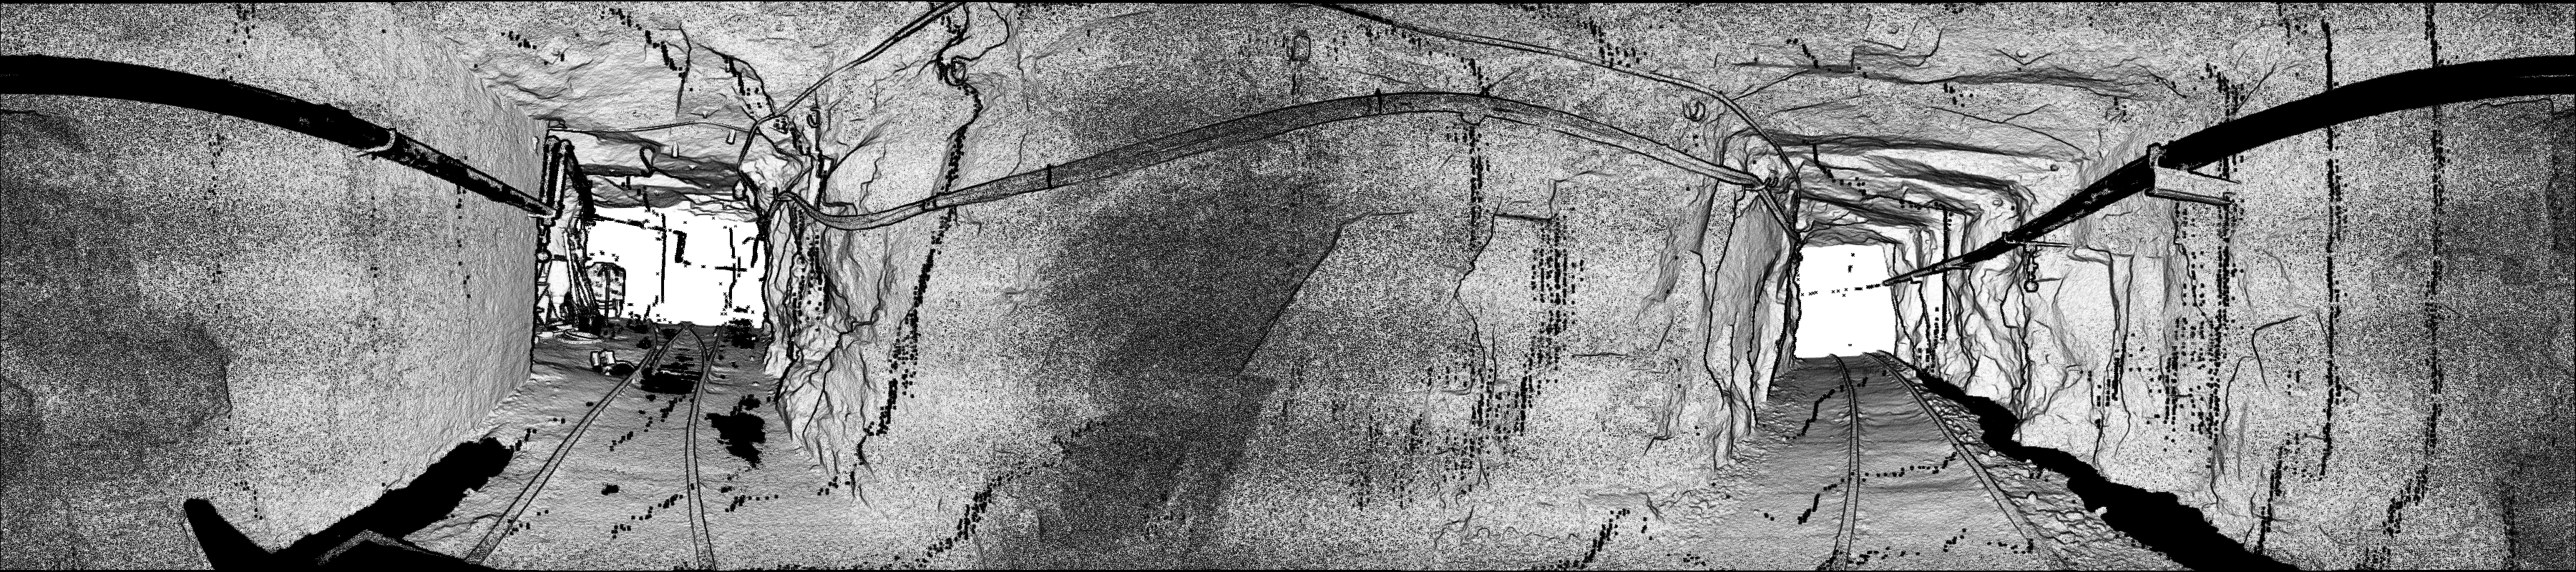
\includegraphics[width=1.0\linewidth]{chapter06/results/conv_images/laserscan/flexion/raw/0000.png}\\
    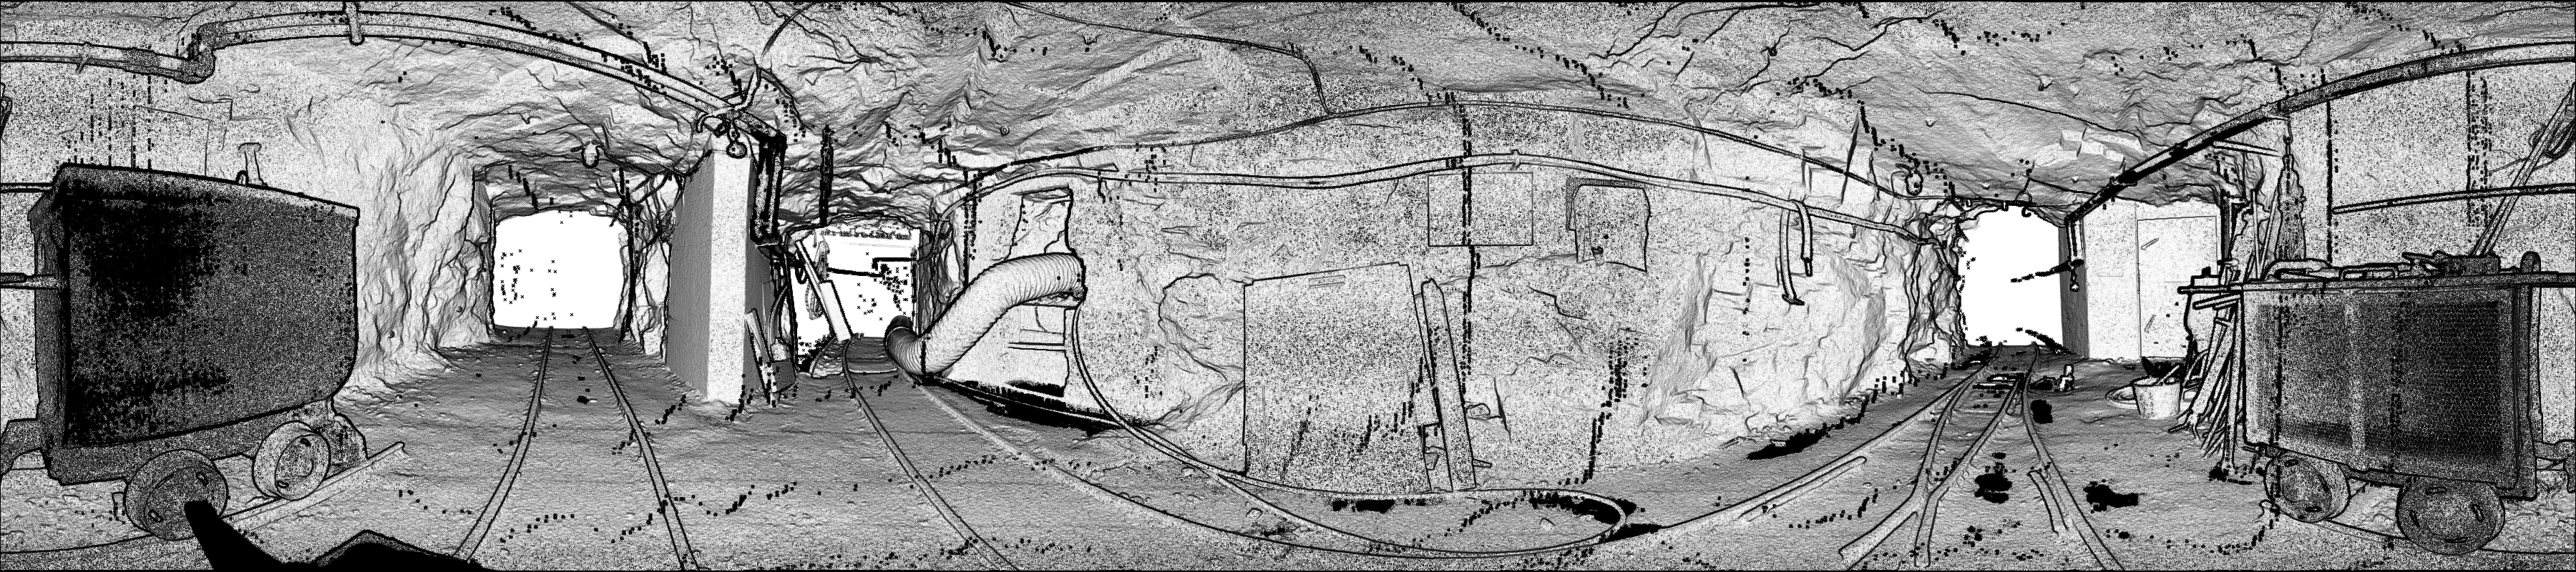
\includegraphics[width=1.0\linewidth]{chapter06/results/conv_images/laserscan/flexion/raw/0002.png}\\
    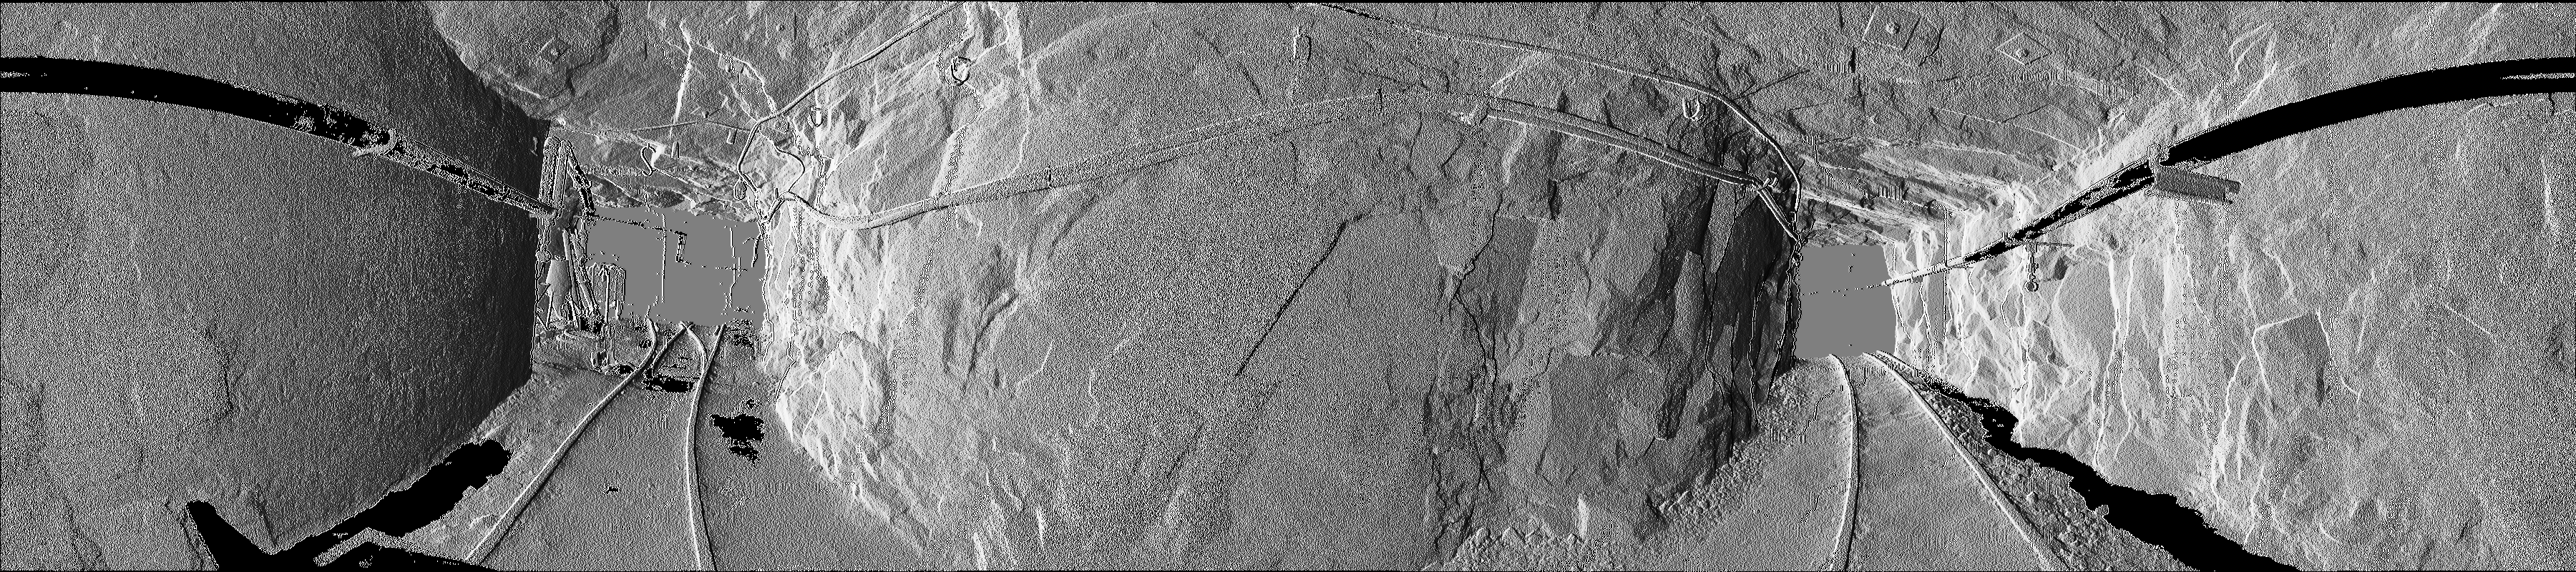
\includegraphics[width=1.0\linewidth]{chapter06/results/conv_images/laserscan/bearing/raw/0000.png}\\
    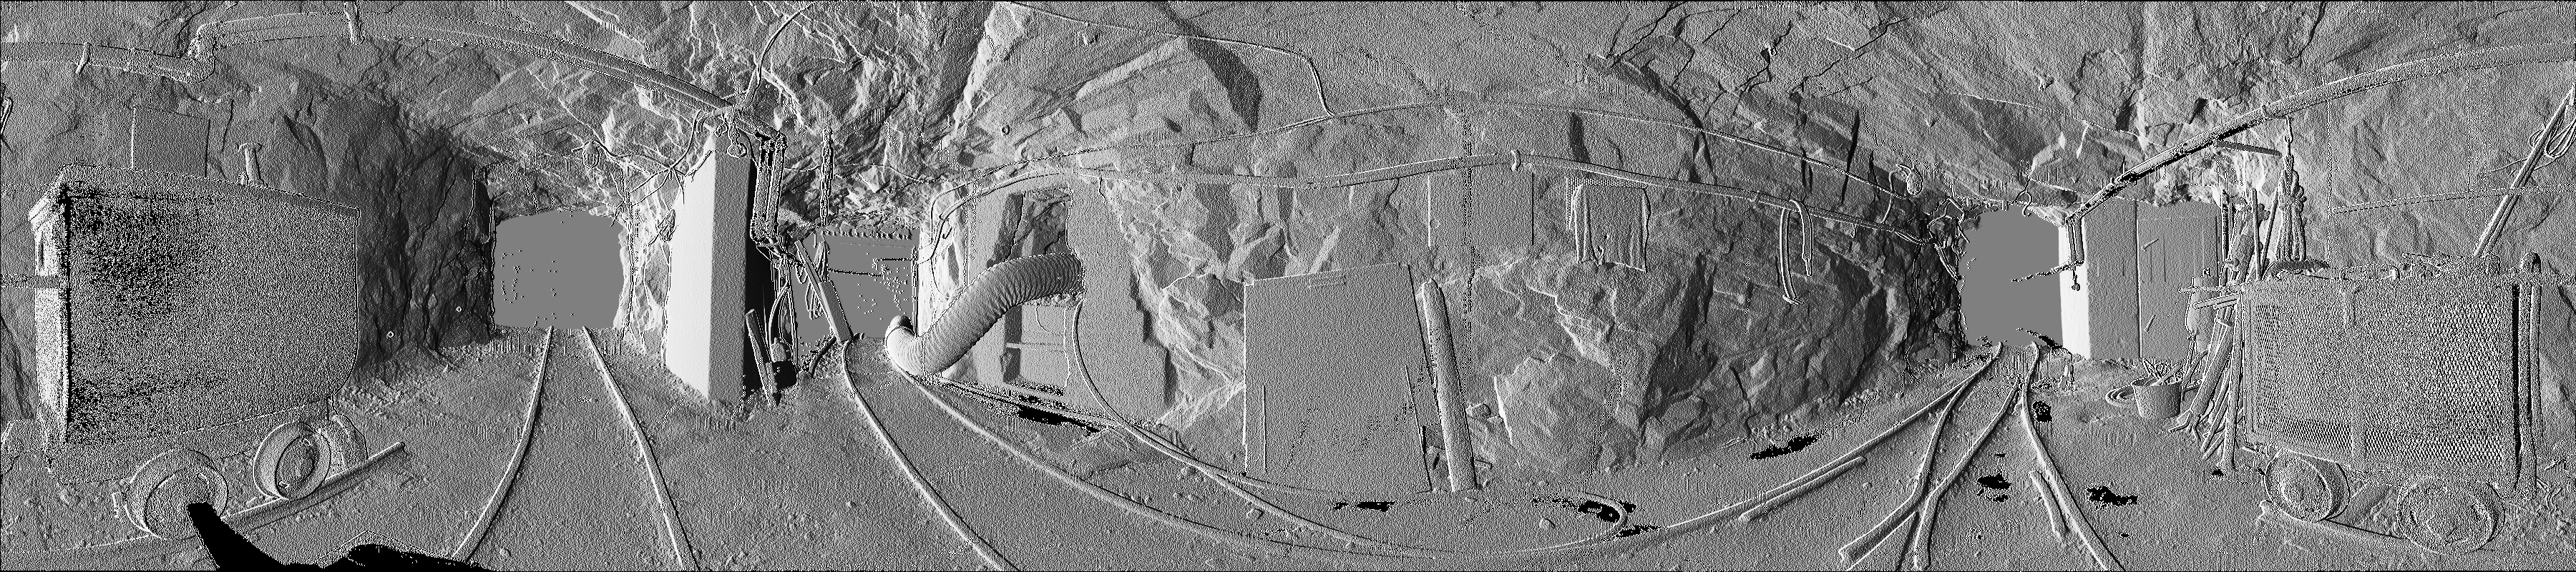
\includegraphics[width=1.0\linewidth]{chapter06/results/conv_images/laserscan/bearing/raw/0002.png}
    \caption{Example \glspl{flexion-image} and \glspl{bearing-angle-image} of the Laserscan dataset without any filtering.}
\end{figure}
\begin{figure}[H]
    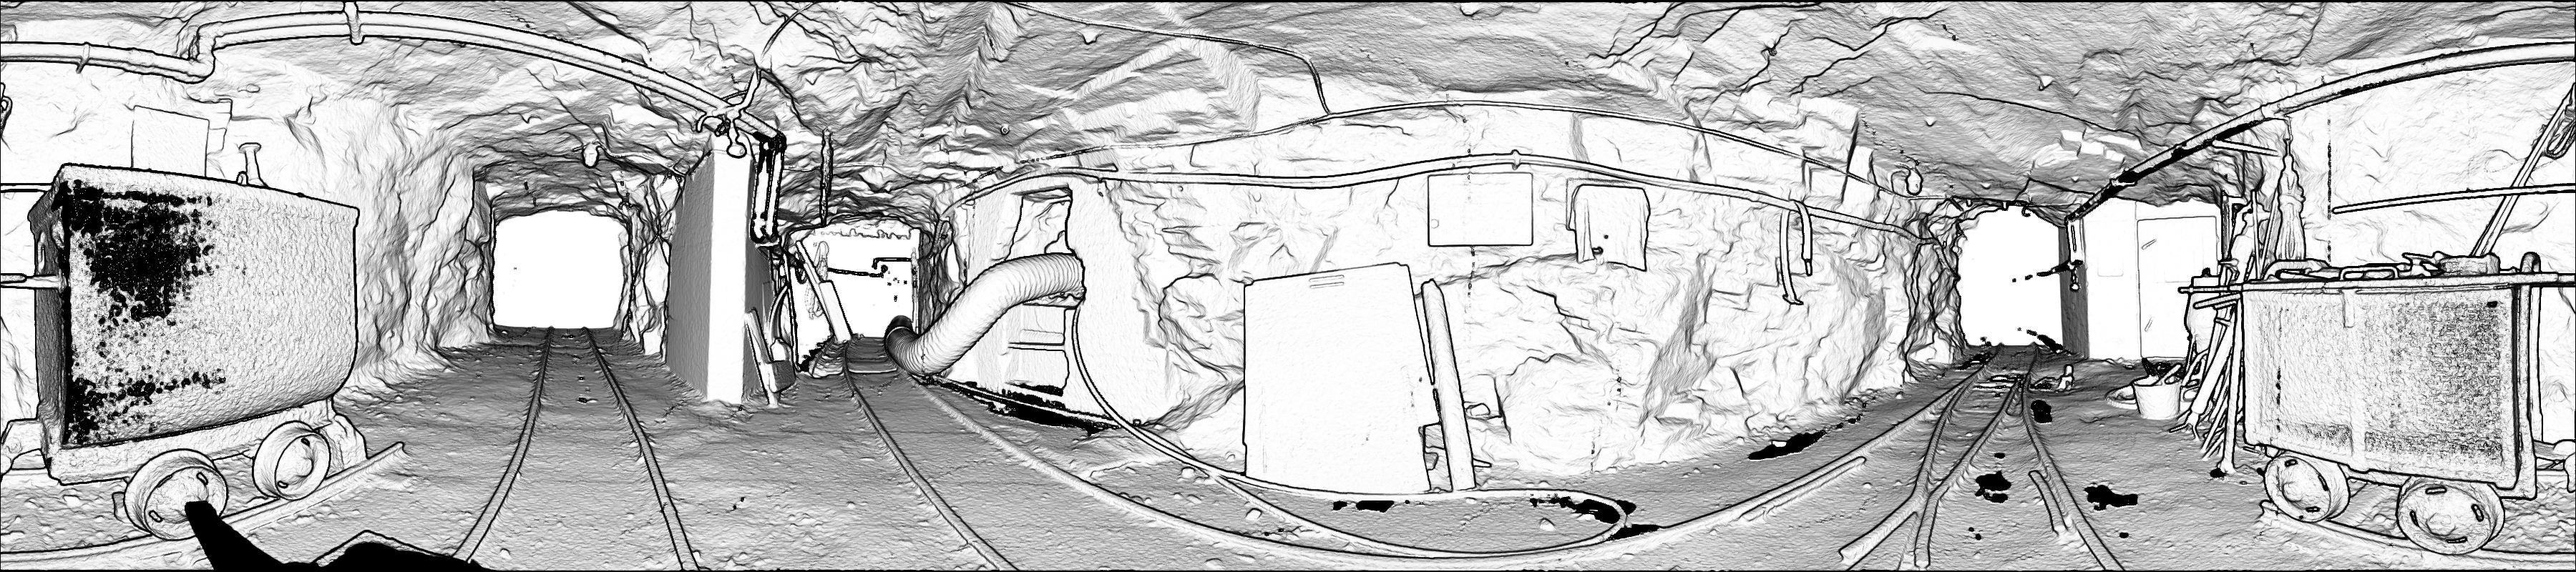
\includegraphics[width=1.0\linewidth]{chapter06/results/conv_images/laserscan/flexion/mb/0002.png}\\
    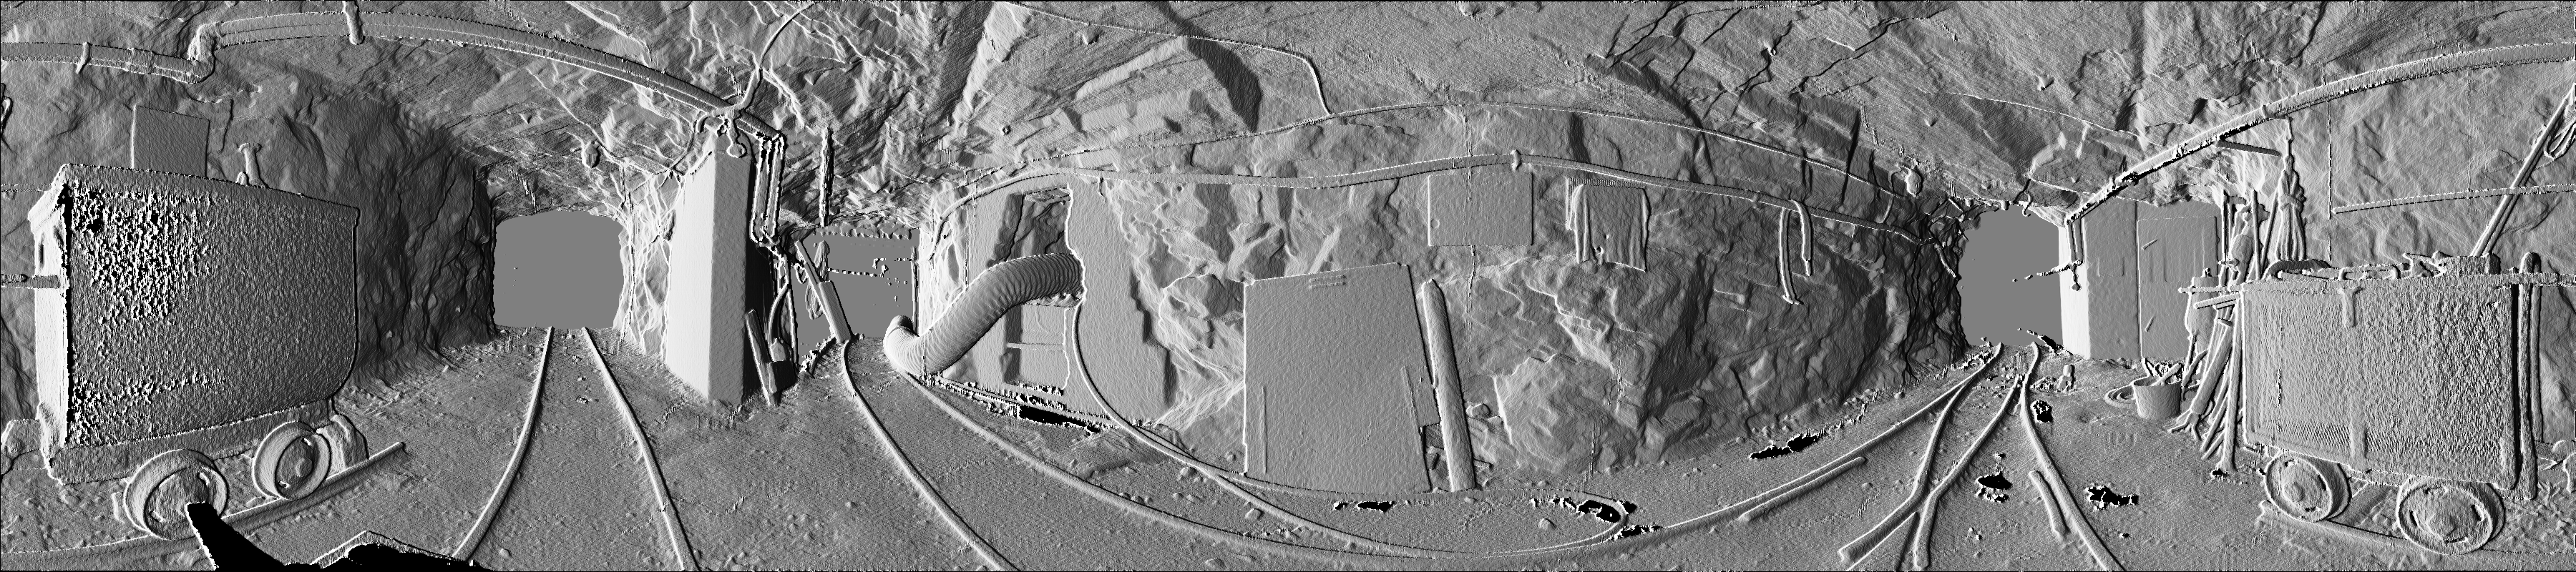
\includegraphics[width=1.0\linewidth]{chapter06/results/conv_images/laserscan/bearing/mb/0002.png}%
    \caption{Filtering the range data with median blur before conversion.}
\end{figure}
\begin{figure}[H]
    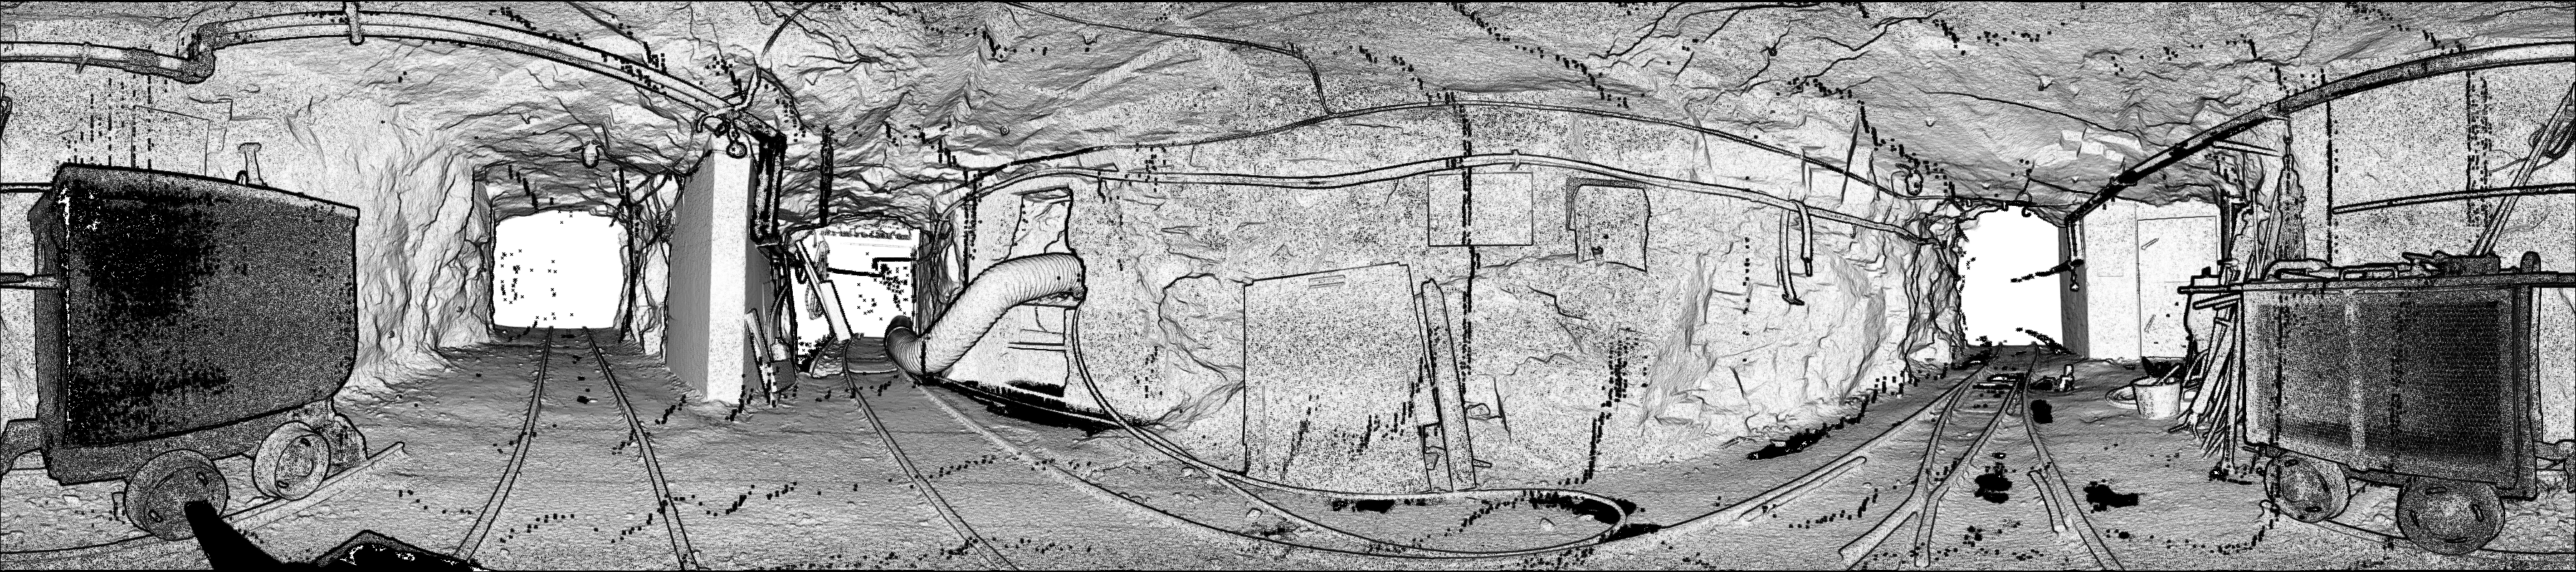
\includegraphics[width=1.0\linewidth]{chapter06/results/conv_images/laserscan/flexion/bl/0002.png}\\
    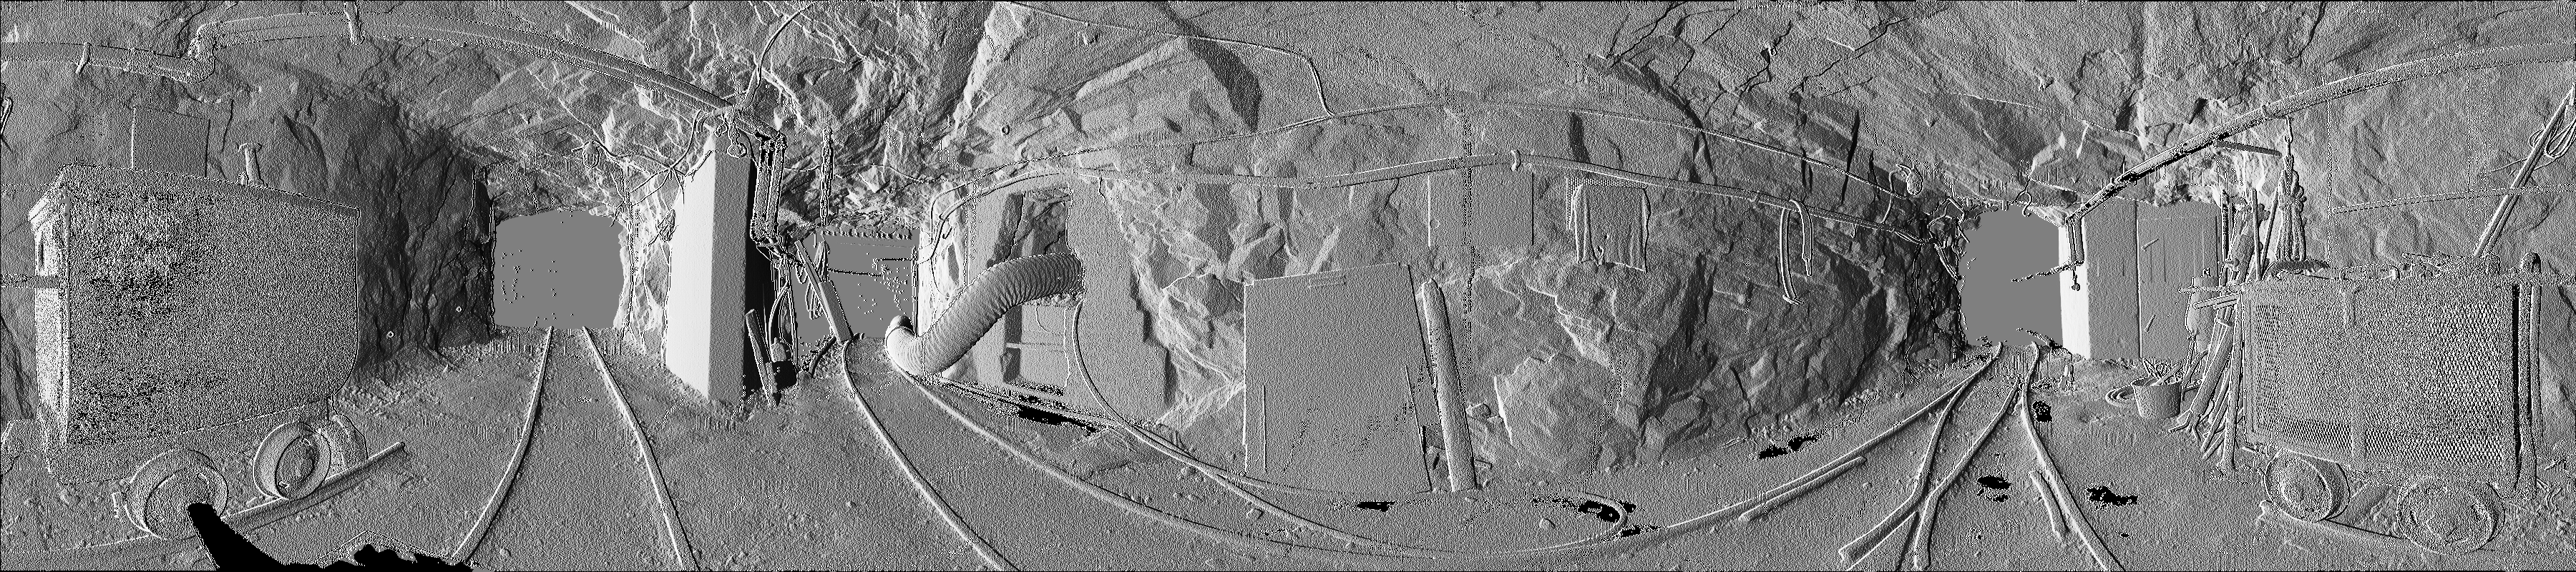
\includegraphics[width=1.0\linewidth]{chapter06/results/conv_images/laserscan/bearing/bl/0002.png}%
    \caption{Filtering the range data with a bilateral filter before conversion.}
\end{figure}
